\chapter[Le basi dello strong gravitational lensing]{Le basi dello strong gravitational \\lensing}
\label{cap:SGL}
Una \emph{lente gravitazionale} è un corpo celeste, tipicamente un ammasso di galassie o una galassia ellittica, ma anche una stella su scale più piccole, che devia la luce proveniente da una sorgente distante e la restituisce all'osservatore in ritardo, deflessa e distorta. In base a quanto si presentano marcati gli effetti, tale fenomeno può essere di tre categorie.
È detto \emph{strong gravitational lensing} quando la lente e la sorgente sono quasi perfettamente allineate lungo la linea di vista, e quindi si formano archi, anelli di Einstein e immagini multiple, ovvero effetti macroscopici forti.
Quello debole, in inglese denominato \emph{weak gravitational lensing}, causa invece distorsioni molto meno marcate, in quanto si ha un allineamento minore e gli effetti sono misurabili solo a livello statistico, analizzando un campione ampio; vi sono poi immagini di sorgenti lontane che non vengono realmente distorte, ma il cui flusso luminoso varia nel tempo ed è talvolta amplificato da oggetti interposti con l'osservatore: è il caso del \emph{microlensing}.

Sebbene, come visto nel Capitolo \ref{cap:cosmologia}, le prime rilevazioni di materia oscura siano avvenute utilizzando effetti di lenti deboli, in questa sezione si approfondirà lo strong gravitational lensing; nel Capitolo \ref{cap:SGL+DM} si mostrerà poi come questo formalismo può essere utilizzato come strumento di indagine per la DM.
\section{Geometria e parametri fondamentali}
Il lensing gravitazionale è una conseguenza diretta della curvatura dello spazio-tempo prevista dalla Relatività Generale. Per descriverne quantitativamente gli effetti è quindi necessario introdurre dapprima l'origine fisica della deflessione della luce e il concetto di angolo di deflessione, da cui deriva il formalismo geometrico della lente gravitazionale.
\subsection{Il principio di Fermat e l'angolo di deflessione}
\label{sez:Fermat-defl}
Il principio di equivalenza della Relatività Generale afferma che, localmente, gli effetti di un campo gravitazionale sono indistinguibili da quelli di un sistema di riferimento accelerato \parencite{Schneider1992}. Si immagini ora un ascensore in caduta libera con un foro su uno dei lati, attraverso il quale filtri un raggio di luce che viaggi da sinistra verso destra. Mentre l'ascensore si muove verso il basso, il raggio colpisce la parete opposta in un punto più basso rispetto a quello da cui era partito: esso apparirà dunque curvato. Combinando questo esperimento mentale con il principio di equivalenza, Einstein si rese conto che la luce doveva poter essere deflessa dalla gravità. Tale deflessione segue le \emph{linee geodetiche}, ovvero le linee che realizzano sulla superficie dello spazio-tempo il percorso di minima lunghezza fra due punti sufficientemente vicini, seguendo la curvatura. Esse possono essere ricavate dalle equazioni di campo di Einstein; ciò che si trova, tuttavia, può essere descritto in maniera equivalente dal \emph{Principio di Fermat}, come in ottica geometrica: il percorso fisicamente realizzato dalla luce rende stazionario il tempo di percorrenza tra due punti.

Si consideri ora un generico indice di rifrazione $n$, in modo da poter definire il tempo di percorrenza della luce in un mezzo come
\begin{equation}
    \int \frac{n}{c}\ dl
\end{equation}
dove $c$ è la velocità della luce nel vuoto e $l$ è il percorso seguito dal raggio.
Poiché tale tempo deve essere un estremale del problema, si cerca un percorso $\vec{\boldsymbol{x}}(l)$ tale per cui 
\begin{equation}
   \delta \int_A^B n(\vec{\boldsymbol{x}}(l))\ dl =0
   \label{eq:var_prob}
\end{equation}
in cui gli estremi A e B sono tenuti fissi. 
Sfruttando la metrica introdotta nel Capitolo \ref{cap:cosmologia} dall'Equazione \ref{eq:FLRW}, e introducendo il campo gravitazionale $\Phi$ attraverso il metodo perturbativo, è possibile ricavare la velocità della luce nel campo gravitazionale 
\begin{equation}
    c'\simeq c\Big(1+\frac{2\Phi}{c^2}\Big) \quad \mathrm{da\ cui} \quad n = \frac{c}{c'}\simeq \Big(1-\frac{2\Phi}{c^2}\Big)
\end{equation}
Un campo gravitazionale può dunque essere trattato come un mezzo con indice di rifrazione variabile.
Per risolvere il problema variazionale introdotto dall'Equazione \ref{eq:var_prob}, si trovano le equazioni di Eulero-Lagrange in funzione di $\vec e$, vettore unitario tangente al raggio luminoso, e dell'indice di rifrazione $n$. La soluzione permette di trovare un'approssimazione per $\dot{\vec e}$
\begin{equation}
    \dot{\vec e}=\frac{de}{d\lambda}= \vec \nabla_\perp \mathrm{ln}\ n \simeq -\frac{2}{c^2}\vec \nabla_\perp \Phi
\end{equation}
dove $\lambda$ è legato alla parametrizzazione della curva.

Poiché $\dot{\vec e}$ rappresenta la variazione infinitesima della direzione di propagazione del raggio luminoso, la deflessione totale si ottiene integrando tale variazione lungo la traiettoria del fotone. Per convenzione, il vettore di deflessione $\hat \alpha$
 è definito come opposto della variazione del versore tangente, così da risultare diretto verso la lente. Si ottiene quindi
 \begin{equation}
     \hat \alpha =\frac{2}{c^2}\int_{\lambda_A}^{\lambda_B}\vec \nabla_\perp \Phi \ d\lambda
 \end{equation}
che rappresenta l'effetto cumulativo del campo gravitazionale della distribuzione di massa della lente sulla direzione di propagazione della luce.

L'equazione in questa forma è però di scarsa utilità, perché richiede di integrare sul percorso del raggio luminoso deflesso, ovvero quello che si sta cercando di ricavare. Poiché la perturbazione $\Phi /c^2\ll 1$, si è soliti quindi adottare l'\emph{approssimazione di Born}, un approccio perturbativo che permette di utilizzare il campo incidente invece del campo totale, purché la perturbazione sia piccola. Come conseguenza, è possibile integrare sul percorso del raggio di luce imperturbato; in funzione del parametro d'impatto $b$ si ha dunque 
 \begin{equation}
     \hat \alpha(b) =\frac{2}{c^2}\int_{-\infty}^{+\infty}\vec \nabla_\perp \Phi \ dz
 \end{equation}
 dove $z$ è la direzione del raggio prima che venga deflesso.
 La disposizione geometrica è rappresentata schematicamente in Figura \ref{fig:geometry}.
 \begin{figure}
     \centering
     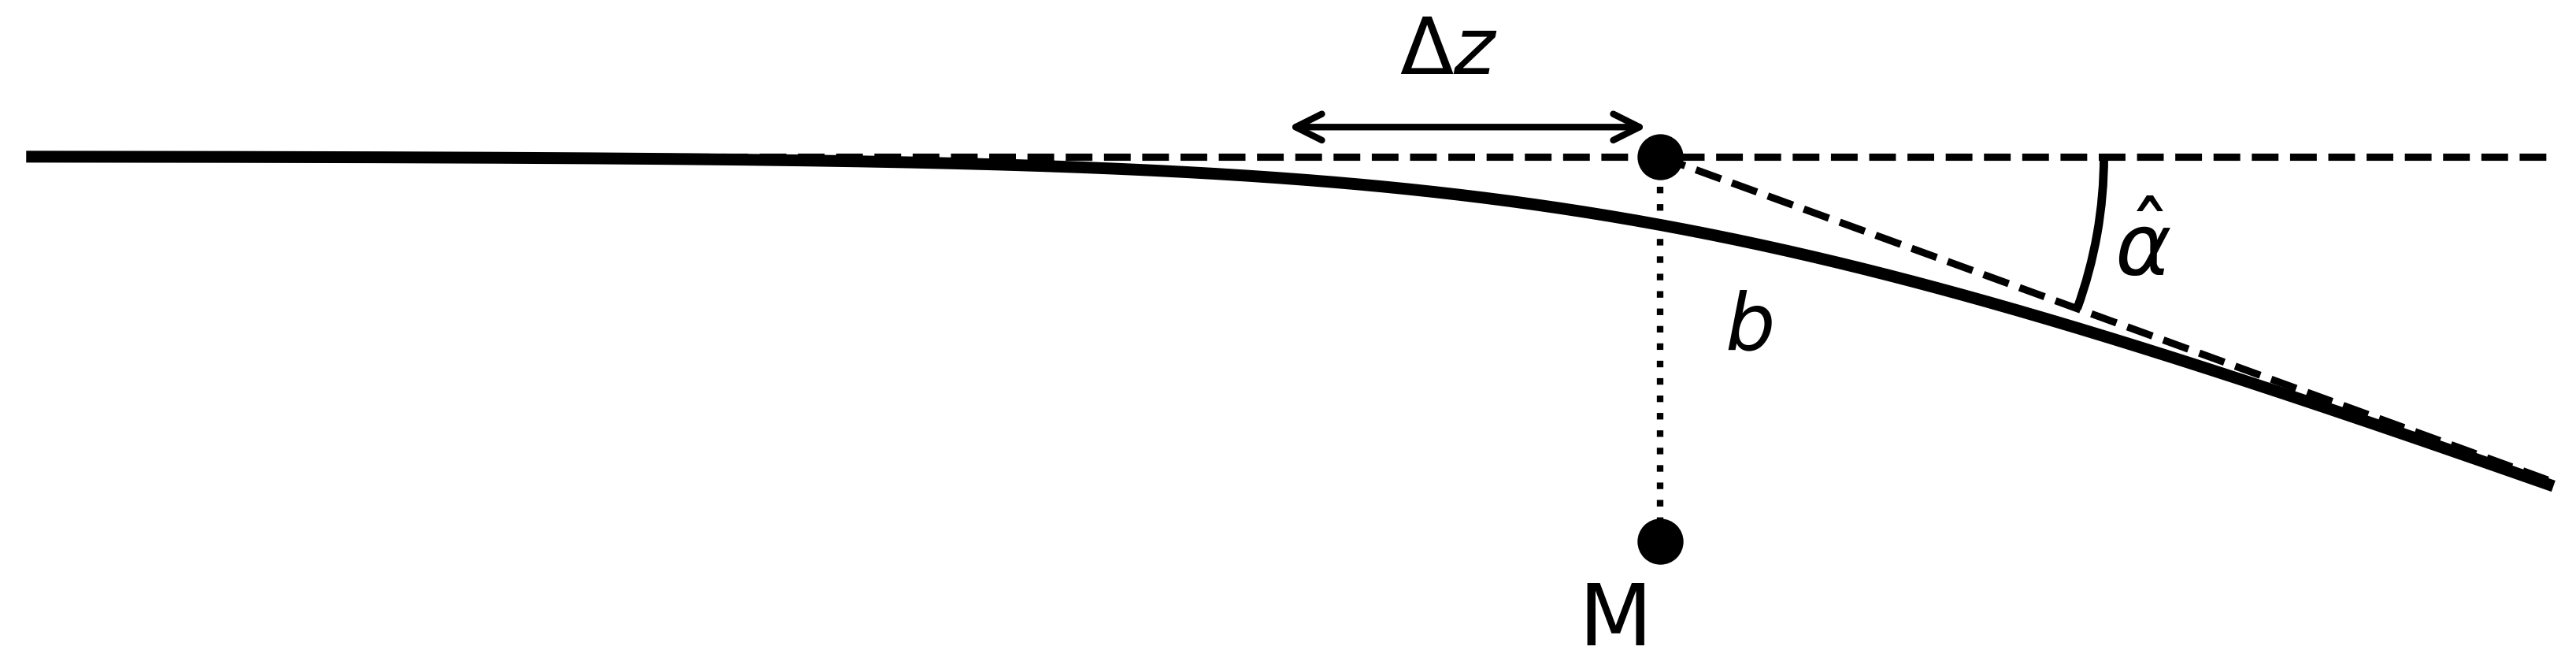
\includegraphics[width=0.6\linewidth]{Immagini/2-Lensing/deflection_horizontal.png}
     \caption{Rappresentazione schematica della geometria del raggio deflesso. Se il raggio viaggia lungo l'asse $z$ con parametro d'impatto $b$, la massa $M$ causa una deviazione di un angolo $\hat \alpha$.}
     \label{fig:geometry}
 \end{figure}

 L'equazione precedente è totalmente generale e descrive la deflessione causata da una distribuzione arbitraria di massa. In linea di principio, il calcolo richiederebbe la conoscenza del potenziale gravitazionale tridimensionale lungo l'intera traiettoria del fotone. Tuttavia, nella maggior parte dei contesti astrofisici, la profondità della lente è trascurabile rispetto alle distanze che la separano dalla sorgente e dall'osservatore: la deviazione avviene quindi in una regione spaziale molto limitata e può essere considerata istantanea.  Questa osservazione giustifica l'introduzione dell'\emph{approssimazione di lente sottile}, descritta nel prossimo paragrafo.
 \newline
\subsection{L'equazione della lente}
Quando le dimensioni fisiche della lente sono trascurabili rispetto alla distanza tra sorgente, lente e osservatore, tutta la sua massa viene proiettata su un piano; tale approssimazione prende il nome di \emph{approssimazione di lente sottile} e il piano su cui viene proiettata la massa della lente prende il nome di \emph{piano della lente}.  In maniera analoga, la distribuzione di massa della sorgente viene proiettata sul \emph{piano della sorgente}.

Introducendo questa approssimazione, la distribuzione di massa della lente è completamente descritta dalla \emph{densità superficiale di massa}
\begin{equation}
    \Sigma(\vec \xi)= \int \rho(\vec \xi, z)\ dz
    \label{eq:sigma}
\end{equation}
dove si è indicato con $\vec \xi$ un generico vettore bidimensionale appartenente al piano della lente, mentre $\rho(\vec \xi, z)$ è la densità di massa tridimensionale.

Per comprendere come si ricava l'angolo di deflessione di una distribuzione continua, conviene partire dal caso di una massa puntiforme, dove il potenziale dipende linearmente dalla massa che lo genera secondo la formula
\begin{equation}
    \Phi(r)=-\frac{GM}{r} \quad \text{da cui} \quad |\hat \alpha(b)|= \frac{4GM}{c^2 b}
\end{equation}
Poiché il potenziale gravitazionale dipende linearmente dalla massa, anche il gradiente del potenziale, e quindi l'angolo di deflessione, obbediscono al principio di sovrapposizione. La deflessione prodotta da una distribuzione di massa arbitraria può quindi essere ottenuta sommando il contributo dei singoli elementi di massa puntiformi, definendo dapprima
\begin{equation}
   d \hat \alpha(\vec \xi)= \frac{4G}{c^2} \frac{(\vec \xi-\vec \xi') }{|\vec \xi-\vec \xi'|^2}dM
   \label{eq:dalpha}
\end{equation}
dove il parametro d'impatto è stato generalizzato al vettore bidimensionale $\vec \xi-\vec \xi'$
 nel piano della lente, 
 poi l'elemento di massa infinitesimo come $dM= \Sigma(\vec \xi')\ d^2 \xi'$. Sostituendolo in \ref{eq:dalpha} e integrando si ha
\begin{equation}
    \hat \alpha(\vec \xi)=\frac{4G}{c^2}\int \frac{(\vec \xi-\vec \xi')\ \Sigma(\vec\xi')}{|\vec \xi-\vec \xi'|^2}\ d^2 \xi'
    \label{eq:defl_angle}
\end{equation}
Le coordinate senza apice sono riferite al raggio luminoso, mentre quelle con l'apice sono legate all'elemento di massa.
Una rappresentazione schematica di un tipico sistema di lente gravitazionale, in cui sia presente anche l'angolo di deflessione, è riportata in Figura \ref{fig:source-lens-plane}, riprodotta da \textcite{Bartelmann2001}.
\begin{figure}
    \centering
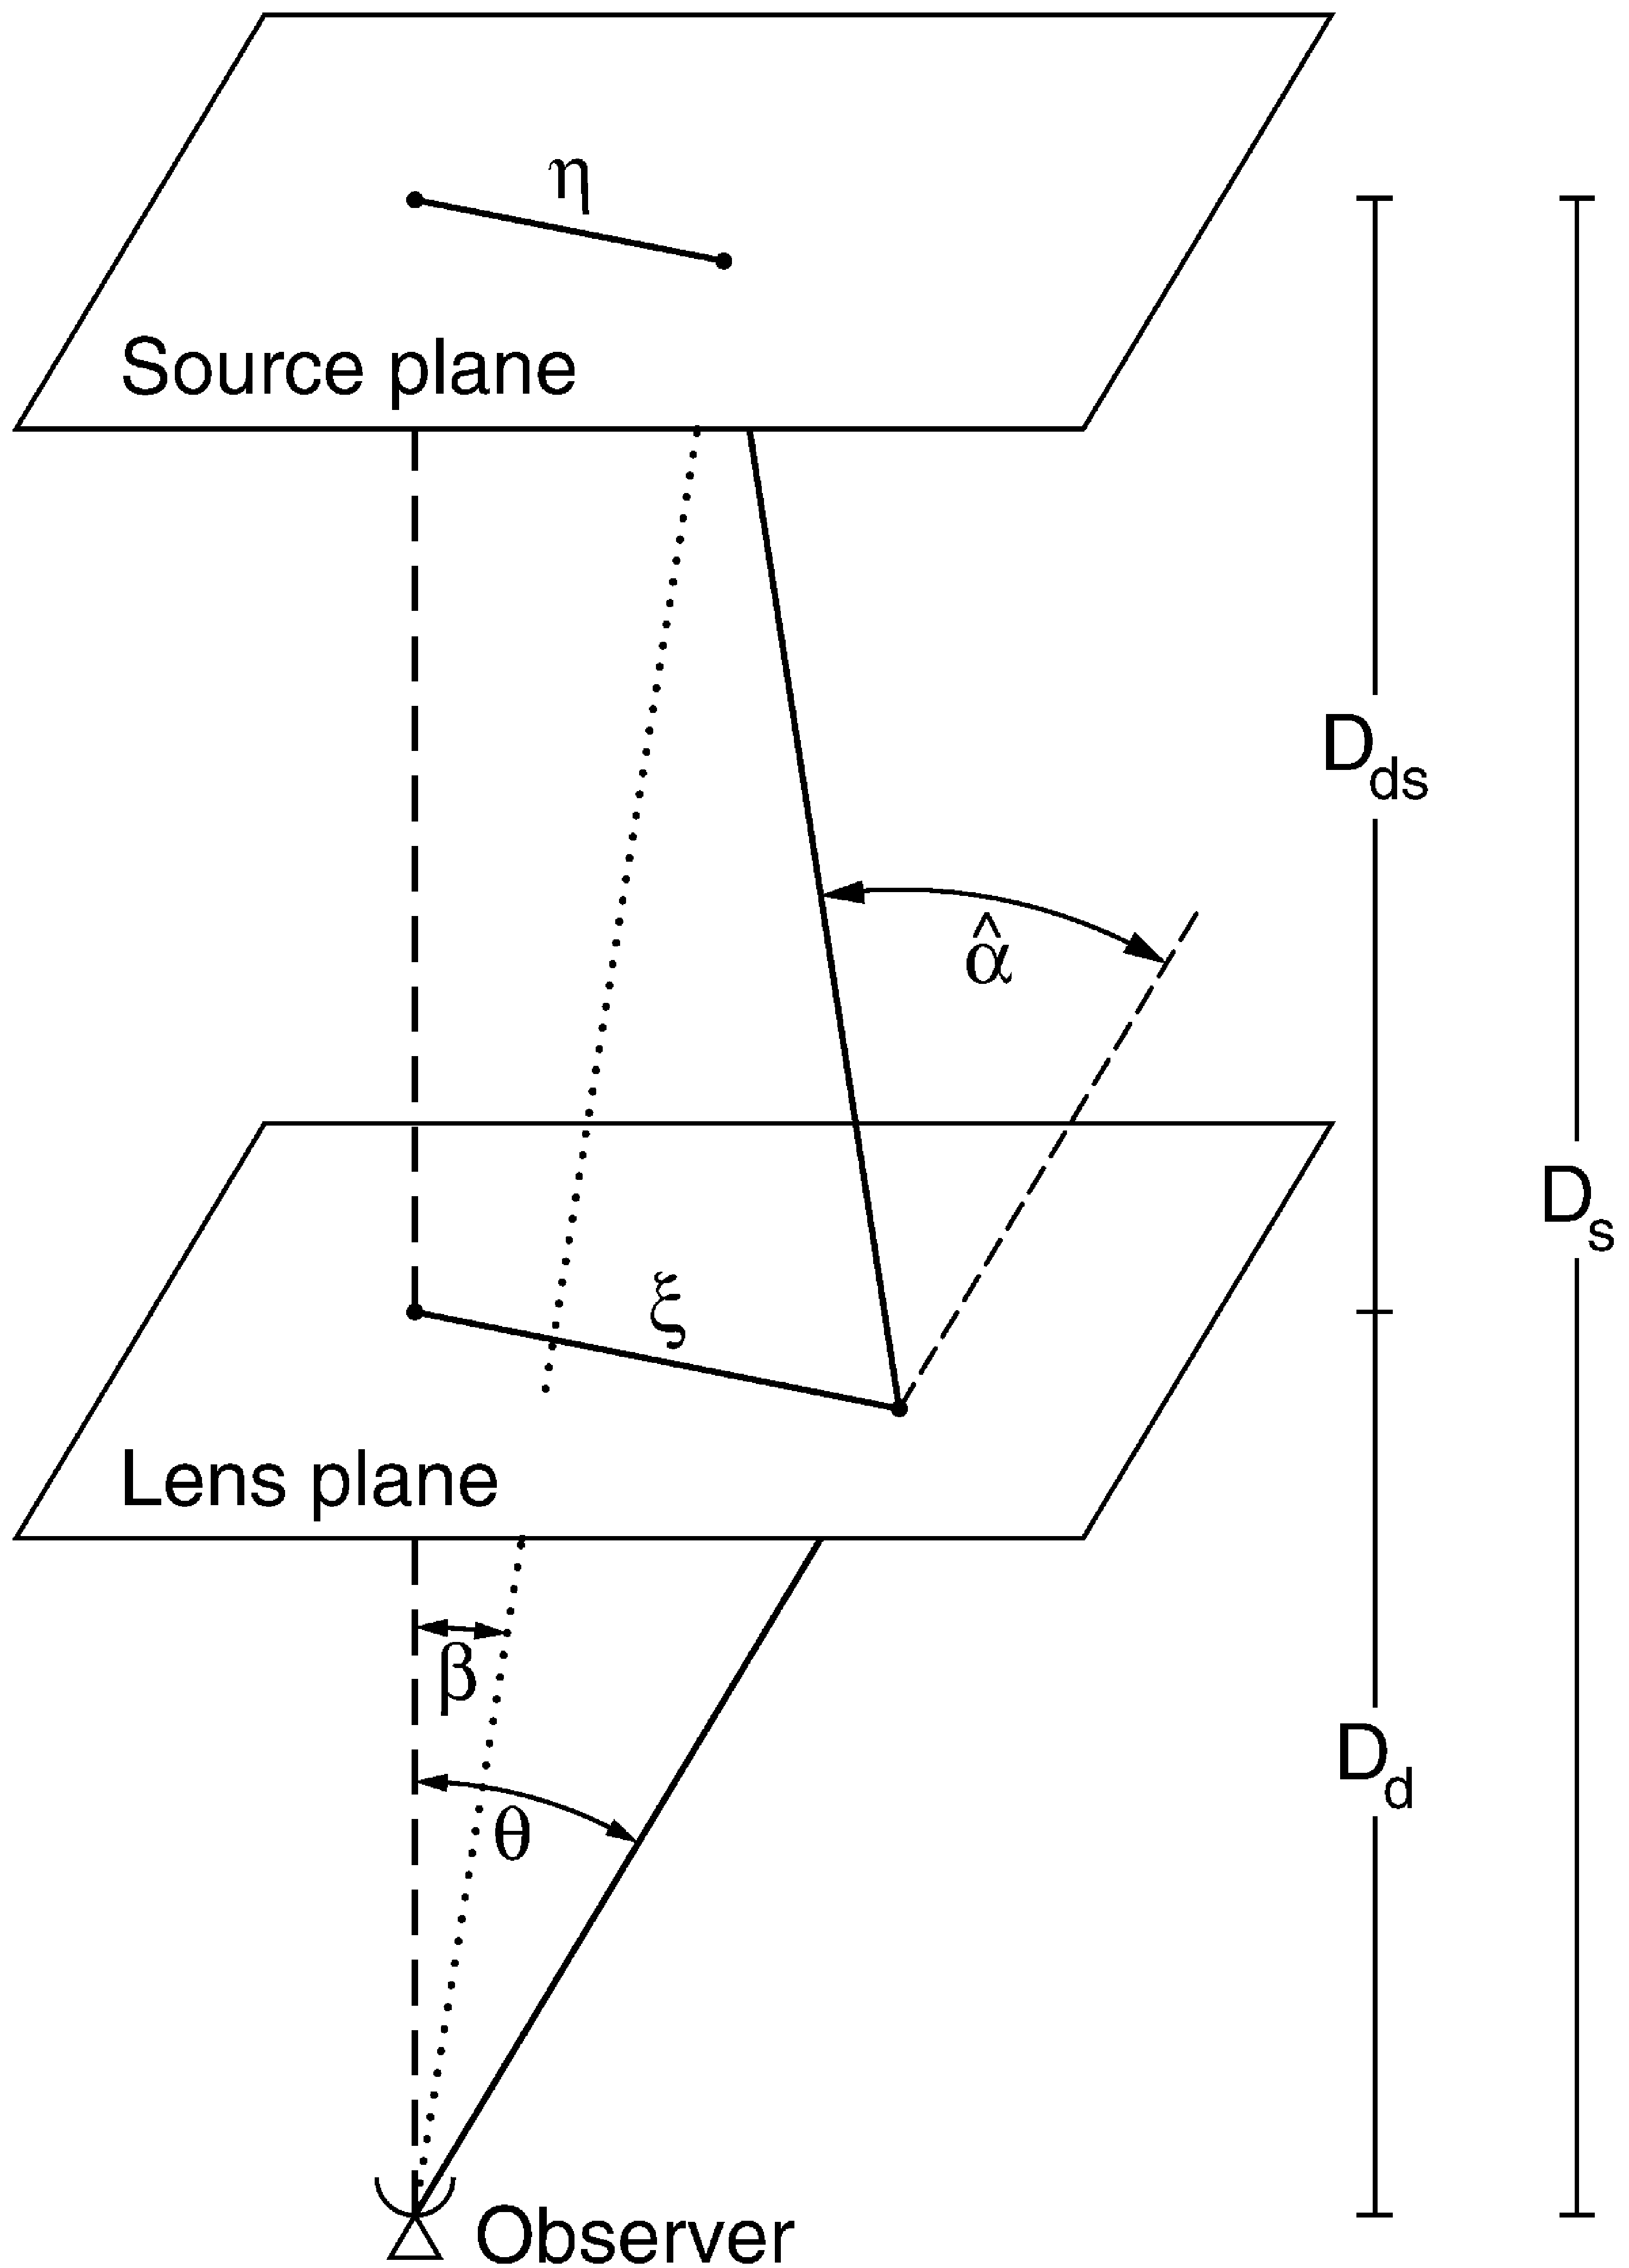
\includegraphics[width=0.4\linewidth]{Immagini//2-Lensing/lens-source-planes.png}
    \caption{Rappresentazione schematica di un tipico sistema di lente gravitazionale; immagine riprodotta da \textcite{Bartelmann2001}.}
    \label{fig:source-lens-plane}
\end{figure}
La lente è collocata a distanza angolare $D_d$ dall'osservatore (dall'inglese \textit{angular diameter distance}) e deflette la la luce proveniente dalla sorgente a distanza angolare $D_s$. La linea tratteggiata che parte dall'osservatore ed è perpendicolare ai due piani della lente e della sorgente prende il nome di \emph{asse ottico}. Le distanze sui due piani si misurano in riferimento ad esso, e sono indicate rispettivamente con $\vec \xi$ per la lente e $\vec \eta$ per la sorgente. Le relative posizioni angolari sono misurate da $\vec \beta$ e $\vec \theta$, in modo che valgano le relazioni $\vec \eta = \vec \beta D_s$ e $\vec \xi = \vec \theta D_d$.

Poiché nel regime astrofisico di interesse le dimensioni trasverse del sistema sono molto inferiori alle distanze tra osservatore, lente e sorgente, si può applicare l'approssimazione dei piccoli angoli. In questo caso, esiste una relazione semplice tra la posizione reale della sorgente nel cielo e quella osservata, che prende il nome di \emph{equazione della lente}
\begin{equation}
    \vec \theta D_s = \vec \beta D_s + \hat \alpha D_{ds} \implies \vec \beta (\vec \theta) = \vec \theta - \hat \alpha (D_d\vec\theta)\frac{D_{ds}}{D_s} 
    \label{eq:lens_eq}
\end{equation}
dove si è definita con $D_{ds}$ la distanza angolare tra sorgente e lente.
Per semplificare la formula, si definisce la \emph{deflessione ridotta}
\begin{equation}
  \hat{\alpha}(\vec\theta)\equiv \frac{D_{ds}}{D_s} \hat \alpha( D_d\vec\theta) 
\end{equation}
cosicché
\begin{equation}
    \vec \beta (\vec \theta) = \vec \theta - \hat \alpha (\vec\theta) 
\label{eq:lens_eq_real}    
\end{equation}
Nell'Equazione \ref{eq:defl_angle} l'angolo di deflessione è espresso in funzione della distribuzione di massa della lente, mentre l'Equazione \ref{eq:lens_eq} lo collega alla posizione apparente delle immagini osservate e a quella reale della sorgente. 
Combinandole fra loro risulta evidente che, attraverso lo studio delle immagini prodotte dall'effetto di lensing, si possono ottenere informazioni sia sulla distribuzione di massa della lente sia sulle proprietà della sorgente. Sebbene, in linea di principio, si possano considerare direttamente gli angoli di deflessione, tale formulazione risulta sconveniente sia dal punto di vista analitico che da quello computazionale. Nelle applicazioni pratiche si preferisce introdurre una nuova grandezza scalare, detta \emph{potenziale della lente}, dal quale l'angolo di deflessione può essere ricavato tramite semplici derivate. Tale formulazione costituisce la base per definire le principali quantità utilizzate nello studio dello strong gravitational lensing, come la convergenza, il fattore di ingrandimento e la distorsione delle immagini, ma anche per prevederne la molteplicità e la posizione. 

\section{Il potenziale della lente}
\label{sez:lensing_potential}
Ogni distribuzione di massa estesa è caratterizzata da un potenziale gravitazionale $\Phi$, tridimensionale e definito in ogni punto dello spazio. I raggi di luce, però, attraversano la distribuzione di massa lungo una traiettoria quasi rettilinea. Di conseguenza, la deflessione non dipende dal valore locale del potenziale gravitazionale, bensì dall'effetto cumulativo esercitato dal suo gradiente lungo la linea di vista.
Per questo motivo si definisce il \emph{potenziale efficace della lente} come
\begin{equation}
    \hat \Psi (\vec \theta)=\frac{2}{c^2}\frac{D_{ds}}{D_dD_s}\int \Phi(D_d\vec \theta, z)\ dz
\end{equation}
Esso è ottenuto proiettando il potenziale gravitazionale lungo la linea di vista e tenendo conto delle distanze relative tra osservatore, lente e sorgente. Il termine \emph{efficace} sottolinea che questa quantità non coincide con il potenziale gravitazionale tridimensionale della lente, ma rappresenta una proiezione opportunamente pesata dai fattori geometrici del sistema. Esso contiene quindi tutta l'informazione necessaria a descrivere la deflessione gravitazionale osservata.

La deflessione ridotta, infatti, può essere ricavata dal potenziale efficace calcolandone il gradiente rispetto alle coordinate angolari
\begin{equation}
  \hat{\alpha}(\vec\theta)=\vec\nabla\hat\Psi(\vec\theta) 
\end{equation}

Nel seguito, si definiscono in maniera unificata le principali quantità impiegate nello studio del lensing gravitazionale, quali la convergenza, l'ingrandimento e la distorsione, tutte ricavabili dal potenziale efficace. Si mostrerà inoltre come la forma del potenziale determini le proprietà delle immagini osservate e si presenterà infine il modello di lente più utilizzato nello strong lensing, ovvero quello isotermo ellittico.

\subsection{Convergenza, magnificazione e distorsione}
\label{sez:convergence, magnification, shear}
Dapprima, soffermiamoci ad analizzare i cambiamenti locali indotti dalla presenza della lente. 
In analogia con le lenti ottiche, anche per quelle gravitazionali è possibile definire la \emph{convergenza}, ovvero il potere focalizzante della massa coinvolta. Essa è funzione dei parametri geometrici del problema e si definisce come variabile adimensionale tramite il rapporto
\begin{equation}
    \kappa(\vec \theta)\equiv \frac{\Sigma(\vec \theta)}{\Sigma_c}
    \label{eq:convergence}
\end{equation}
dove si è introdotta la \emph{densità superficiale critica}
\begin{equation}
    \Sigma_c=\frac{c^2}{4\pi G}\frac{D_s}{D_dD_{ds}}
    \label{eq:sigma_c}
\end{equation}
Tale densità caratterizza la lente e corrisponde alla condizione $\hat \alpha(\vec\theta)=\vec\theta$, ovvero quella in cui osservatore e sorgente sono perfettamente allineati; in questo caso, l'immagine di un singolo raggio luminoso si forma esattamente al corrispondente angolo di deflessione.

La convergenza misura dunque quanta massa è presente lungo la linea di vista rispetto a quanta sarebbe necessaria per produrre un effetto di strong lensing (ad esempio, immagini multiple o archi): le regioni in cui tali effetti si verificano, infatti, sono generalmente associate a convergenze dell'ordine dell'unità.

Nel nuovo formalismo che stiamo introducendo, la convergenza è proporzionale al laplaciano del potenziale della lente 
\begin{equation}
    \kappa(\vec\theta)=\frac{1}{2}\nabla^2\hat\Psi(\vec\theta)
    \label{eq:conv_pot}
\end{equation}
Tale equazione può essere derivata sostituendo la \ref{eq:sigma_c} e la \ref{eq:sigma} (con opportuno cambio di variabile) nell'Equazione \ref{eq:convergence} e combinando il risultato ottenuto con l'equazione di Poisson, espressa nelle dovute coordinate. Fisicamente, essa afferma che maggiore è la curvatura locale del potenziale della lente (pensato come superficie bidimensionale), o, in altri termini, maggiore è la concentrazione di massa, tanto più efficacemente la lente stessa riesce a focalizzare  i raggi luminosi. 

La deviazione dei fotoni ad opera di una distribuzione di massa dà dunque origine a immagini più grandi e luminose, ma anche deformate. Infatti, nel caso in cui la sorgente presenti un'estensione, come avviene nella realtà, ogni raggio di luce è deflesso in modo differenziale e indipendente dagli altri. 
La separazione angolare tra osservatore e sorgente, per sorgenti piccole, può essere linearizzata al prim'ordine
\begin{equation}
    d\vec\beta(\vec\theta)= \mathbf{A}\ d\vec\theta 
\end{equation}
dove si è definita la \emph{matrice jacobiana della trasformazione} come
\begin{equation}
   A_{ij}=\frac{\partial \beta_i}{\partial \theta_j}
   \label{eq:jacobian_matrix}
\end{equation}
Derivando l'Equazione della lente trovata in \ref{eq:lens_eq} rispetto a $\vec\theta$ ed esprimendo la deflessione ridotta in termini di potenziale della lente si trova 
\begin{equation}
    \mathbf{A}(\vec\theta)= \mathbb{I}- \mathbf{\Psi} \quad \text{con} \quad \mathbf{\Psi}=\vec\nabla(\vec\nabla\hat\Psi) \equiv \begin{pmatrix}
        \Psi_{11} & \Psi_{12}\\
        \Psi_{21} & \Psi_{22}
    \end{pmatrix}
    \quad \text{e} \quad \Psi_{ij}\equiv \frac{\partial^2\hat\Psi}{\partial \theta_i \partial \theta_j}
\end{equation}
A questo punto è utile riesprimere la matrice come composizione di una parte puramente \emph{isotropa}, che cambia localmente la dimensione dell'immagine mantenendone la forma, e una parte puramente \emph{anisotropa}, che invece la distorce senza cambiare l'area.
Si può dimostrare che la parte isotropa dipende unicamente dalla convergenza, introdotta in precedenza, mentre quella anisotropa dipende da una nuova grandezza, indicata con $\gamma(\vec\theta)$, che in inglese prende il nome di \emph{shear} ed è legata alla distorsione dell'immagine; omettendo le dipendenze dall'angolo
\begin{equation}
    \mathbf{A}=(1-\kappa)\mathbb{I}-\Gamma
\end{equation}
dove si è definita la \emph{shear matrix} (matrice di distorsione) come
\begin{equation}
    \Gamma= \begin{pmatrix}
        \gamma_{11} & \gamma_{12}\\
        \gamma_{21} & \gamma_{22}\\
    \end{pmatrix}=\begin{pmatrix}
        \frac{1}{2}(\Psi_{11}-\Psi_{22}) & \Psi_{12}\\
        \Psi_{12} & \frac{1}{2}(\Psi_{11}-\Psi_{22})\\
    \end{pmatrix}
\end{equation}
Essa è simmetrica e a traccia nulla, dunque è sempre diagonalizzabile con matrici ortogonali. Lo shear $\gamma$ corrisponde agli autovalori di questa matrice, che sono sempre uguali e opposti e dipendono dal punto $\vec\theta$ considerato.
Nella base in cui $\mathbf{A}$ è diagonale, essa assume dunque la forma 
\begin{equation}
     \mathbf{A}=
     \begin{pmatrix}
 1-\kappa-\gamma & 0\\
 0 & 1-\kappa+\gamma
     \end{pmatrix}    
\end{equation}
Concettualmente, il potenziale della lente agisce localmente sulle immagini in due modi: ingrandendole e deformandole. Tale azione locale è matematicamente sintetizzata dalla matrice $\mathbf{A}$, che dipende infatti dai parametri $\kappa$ e $\gamma$. Poiché l'inverso del determinante di una trasformazione è legato alla modifica dei volumi presenti nello spazio in cui tale trasformazione avviene, di definisce \emph{magnificazione} o \emph{fattore di ingrandimento}
\begin{equation}
    \mu=\frac{1}{\det\mathbf{A}}=\frac{1}{(1-\kappa)^2-\gamma^2}
    \label{eq:magnification}
\end{equation}
Il segno indica la parità dell'immagine: un determinante negativo indica che essa è stata ribaltata rispetto alla sorgente originaria. Il valore di $\mu$, invece, indica se e di quanto l'immagine è stata ingrandita o rimpicciolita dall'azione del potenziale della lente.

Quando almeno uno dei due autovalori di $\mathbf{A}$ è nullo, la magnificazione diverge. I punti corrispondenti a $\det\mathbf{A}(\vec\theta)=0$ definiscono una o più curve sul piano della lente, che prendono il nome di \emph{linee critiche}. Attraverso l'equazione della lente, è possibile trovare i corrispondenti punti $\vec\beta$ sul piano della sorgente, i quali danno luogo alle \emph{caustiche}. Entrambe queste linee sono fondamentali nella formazione delle immagini. Un esempio rappresentativo di critiche e caustiche è riportato in Figura \ref{fig:caustics_and_critics}.

\begin{figure}
    \centering
    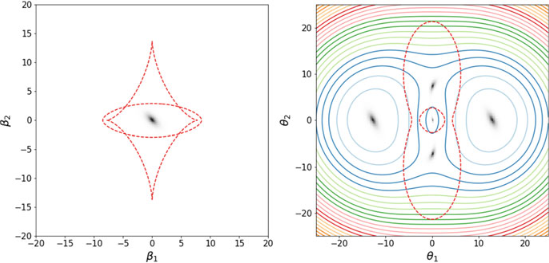
\includegraphics[width=0.8\linewidth]{Immagini//2-Lensing/caustics and critics.png}
    \caption{Esempio della relazione tra caustiche e linee critiche in una lente ellittica. Nel pannello di sinistra sono riportate le caustiche (linee tratteggiate rosse) sul piano della sorgente, insieme alla sorgente rappresentata in nero. Nel pannello di destra sono mostrate le corrispondenti linee critiche sul piano della lente (linee tratteggiate rosse) e le cinque immagini lensate. Le linee continue colorate rappresentano curve a ritardo temporale costante. Immagine riprodotta da \cite{Meneghetti2021}.}
    \label{fig:caustics_and_critics}
\end{figure}

\subsection{Formazione delle immagini}
\label{sez:Image formation}
Finora si sono analizzate unicamente le perturbazioni locali che il potenziale di una lente può generare. Per avere una visione d'insieme, in linea di principio, bisognerebbe risolvere la \ref{eq:lens_eq_real}: per un potenziale arbitrario, l'equazione è non-lineare, dunque ammette soluzioni multiple, e ognuna di esse corrisponde ad un'immagine.
La sua non-linearità, però, la rende spesso anche irrisolvibile analiticamente.

Come visto nel paragrafo \ref{sez:Fermat-defl}, la luce segue cammini che rendono stazionario il tempo di arrivo (Principio di Fermat). In presenza di una lente, i contributi al tempo di arrivo possono essere sia geometrici, legati alla lunghezza differente dei percorsi, che gravitazionali, ovvero influenzati dalla forma di $\Psi$; ciò comporta la possibile presenza di svariati minimi, in ognuno dei quali si forma un'immagine.
Sebbene non si conosca esplicitamente la forma delle soluzioni, se ne possono dunque dedurre alcune proprietà analizzando la forma del potenziale della lente. Nel seguito non verrà approfondita la teoria del tempo di arrivo; ci limiteremo alle conseguenze sulla formazione delle immagini.

Ad ogni punto del piano della lente è associata una funzione di ritardo temporale $t(\vec\theta)$, che può essere vista come una varietà bidimensionale. La matrice hessiana $\mathbf{T}$ di tale superficie, che ne definisce i punti critici, è direttamente proporzionale alla matrice $\mathbf{A}$ introdotta nel paragrafo precedente, la quale può essere analizzata per dedurre le proprietà delle immagini.

Si dicono immagini di \emph{tipo I} quelle che sorgono nei minimi della superficie del tempo di arrivo. Gli autovalori di $\mathbf{T}$ sono entrambi positivi, quindi $\det \mathbf{A}>0$ e tr$\mathbf{A}>0$: poiché la magnificazione è positiva, le immagini hanno la stessa parità della sorgente, e, essendo la curvatura positiva in tutte le direzioni, risultano ingrandite.

Si dicono immagini di \emph{tipo II} quelle che sorgono nei punti di sella della superficie del tempo di arrivo. Gli autovalori di $\mathbf{T}$ hanno segni opposti, quindi $\det \mathbf{A}<0$, mentre il segno della traccia può variare. Poiché la magnificazione è negativa, le immagini hanno parità invertita rispetto alla sorgente.

Infine, si dicono immagini di \emph{tipo III} quelle che sorgono nei massimi della superficie del tempo di arrivo. Gli autovalori di $\mathbf{T}$ sono entrambi negativi, quindi $\det \mathbf{A}>0$ e tr$\mathbf{A}<0$: poiché la magnificazione è positiva, le immagini hanno la stessa parità della sorgente e, essendo la curvatura negativa in tutte le direzioni, risultano rimpicciolite.

 Quando la sorgente e la lente sono perfettamente allineate, i minimi si trovano su un anello, mentre il massimo è posizionato al centro. Quest'ultima immagine, tuttavia, spesso è talmente piccola da risultare invisibile; inoltre, essa può trovarsi sovrapposta alla luce emessa dalla lente, risultando difficile da distinguere. Tale struttura prende il nome di \emph{anello di Einstein}, in inglese \emph{Einstein Ring}, ed è un segno distintivo delle lenti gravitazionali forti. Se ne riporta un esempio in Figura \ref{fig:einstein_ring}. 
 \begin{figure}
    \centering
    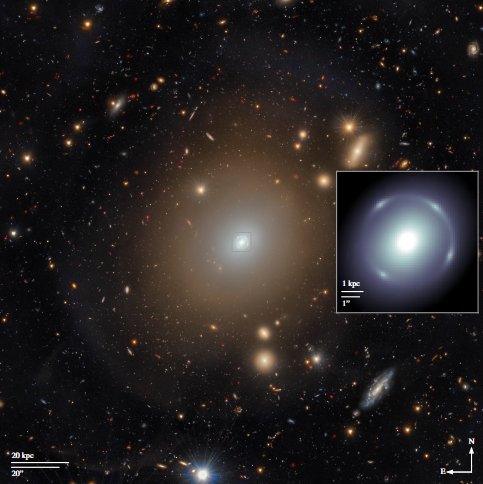
\includegraphics[width=0.5\linewidth]{Immagini//2-Lensing/einstein_ring.png}
    \caption{Esempio di lente gravitazionale forte che produce un anello di Einstein completo. A lato è presente un ingrandimento della zona centrale; il quadrato ha un lato di 8''. Sull'immagine sono riportate le diverse scale fisiche. Immagine riprodotta da \textcite{O_Riordan_2025}.}
    \label{fig:einstein_ring}
\end{figure}

Allontanando la sorgente dall'asse ottico, l'anello tende a rompersi, dando origine a immagini multiple che, per motivi topologici, si presentano sempre in numero dispari. Inoltre, poiché spesso l'immagine nel massimo è difficilmente visibile, anche se in linea di principio si potrebbero avere fino a cinque immagini, il massimo numero osservato nella pratica è quattro. Uno studio più approfondito di come cambia l'insorgere di immagini al variare dei parametri geometrici del sistema sarà studiato nel Capitolo \ref{cap:simulazioni}, dove si simuleranno immagini di sorgenti più o meno allineate rispetto all'osservatore. Una cosa importante da notare fin da subito è però il ruolo delle linee critiche: esse infatti, corrispondendo a zone in cui cambia il segno della curvatura, separano le regioni a molteplicità diversa di immagini.

 La matrice hessiana permette anche di scomporre la curvatura, e dunque il relativo potere di magnificazione, lungo le diverse direzioni del piano; da questo dipende l'ingrandimento o la riduzione tangenziale e trasversale delle immagini.
 Quando una delle due direzioni risulta molto più magnificata dell'altra, si formano i cosiddetti \emph{archi gravitazionali}: in particolare, quelli tangenziali sono uno degli effetti distintivi dello strong gravitational lensing. Un esempio è riportato in Figura \ref{fig:grav_arcs} \parencite{Longair2015}.
 \begin{figure}
     \centering
     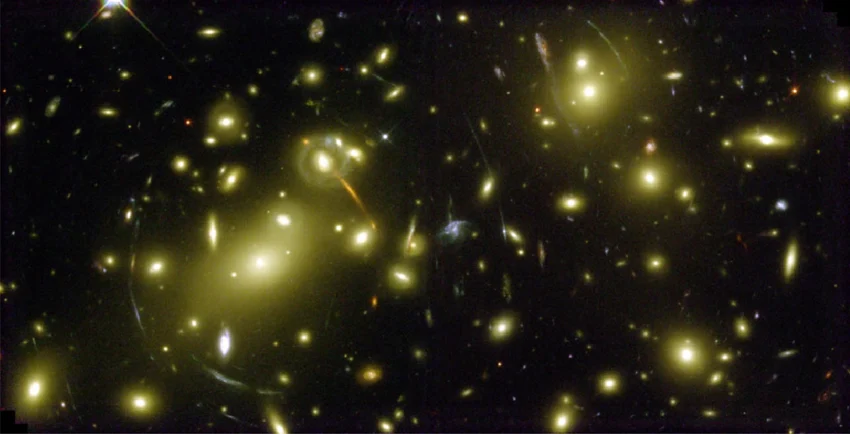
\includegraphics[width=0.75\linewidth]{Immagini/2-Lensing/grav_arcs.png}
     \caption{Esempi di archi gravitazionali tangenziali prodotti da un ammasso di galassie, il quale funge da lente gravitazionale forte. Immagine riprodotta da \textcite{Longair2015}.}
     \label{fig:grav_arcs}
 \end{figure}

Questi fenomeni si verificano in corrispondenza delle curve critiche tangenziali (ovvero i punti per cui $1-\kappa-\gamma=0$) e di quelle radiali (dove $1-\kappa+\gamma=0$). Gli archi tangenziali, più comuni, sono usati per ricostruire il potenziale gravitazionale degli ammassi, e dunque anche la distribuzione di massa barionica e oscura racchiusa  all'interno delle relative linee critiche. Gli archi radiali invece, in genere più rari da osservare, sono sensibili alla pendenza del profilo di densità nelle regioni centrali dell'oggetto studiato e vengono utilizzati per vincolare la distribuzione di materia oscura nel nucleo degli ammassi, contribuendo a fare chiarezza sul \emph{Core-Cusp Problem}.


\subsection{Il modello isotermo ellittico}
Uno dei pochissimi esempi per cui l'equazione della lente è risolvibile analiticamente è il \emph{potenziale isotermo sferico singolare}. Il relativo profilo di densità può essere derivato assumendo che la materia di cui la lente è composta si comporti come un gas perfetto confinato in una buca di potenziale sferica, in equilibrio termico e idrodinamico con l'ambiente esterno. Ciò implica che l'energia cinetica media è costante nello spazio, ovvero la dispersione di velocità $\sigma_v$ è indipendente dalla distanza dal centro $r$. La formula esplicita del profilo di densità è 
\begin{equation}
    \rho_{SIS}(r)=\frac{\sigma_v^2}{2\pi Gr^2}
    \label{eq:rho_SIS}
\end{equation}
dove l'abbreviazione SIS deriva dall'inglese \emph{Singular Isothermal Sphere}. L'aggettivo singolare viene apposto per sottolineare la divergenza per $r=0$, che lo distingue dalla versione \textit{softened}, in cui tale singolarità viene rimossa.
Proiettando la densità tridimensionale lungo la linea di vista, si ottiene il corrispondente profilo della densità superficiale
\begin{equation}
    \Sigma (\xi)=2\frac{\sigma_v^2}{2\pi G}\int_0^\infty\frac{dz}{\xi^2+z^2}=\frac{\sigma_v^2}{2\pi G\xi}
    \label{eq:sup_dens_SIS}
\end{equation}
anch'esso singolare per $\xi = 0$.

Facendo l'opportuno cambiamento di variabile e utilizzando la formula \ref{eq:convergence} si ottiene la convergenza 
\begin{equation}
    \kappa(\theta)=2\frac{\sigma_v^2\pi D_{ds}}{\theta c^2 D_s}=\frac{\theta_E}{2\theta}
    \label{eq:SIS_kappa}
\end{equation}
dove si è introdotto come parametro il \emph{raggio di Einstein}, per raccogliere tutta la dipendenza dalla massa della lente e dalla geometria del sistema in un unico valore.
\begin{equation}
    \theta_E=\frac{4\pi\sigma_v^2}{c^2}\frac{D_{ds}}{D_s}
    \label{eq:einstein_radius}
\end{equation}
Integrando due volte si ottiene dunque il potenziale isotermo sferico circolare
\begin{equation}
    \hat\Psi(\theta)=\theta_E|\theta|
    \label{eq:SIS}
\end{equation}
Da questo è possibile ricavare dapprima l'angolo di deflessione
\begin{equation}
    \hat\alpha(\theta)=\theta_E\frac{\vec\theta}{|\theta|}
\end{equation}
e poi l'equazione della lente
\begin{equation}
    \vec\beta=\vec\theta-\theta_E\frac{\vec\theta}{|\theta|}
\end{equation} 
che può essere riscritta in forma scalare sfruttando la simmetria assiale del problema e introducendo la funzione segno
\begin{equation}
    \beta=\theta-\theta_E\ \text{sign}(\theta)
\end{equation}
Quando sorgente e osservatore sono allineati tra loro, ovvero $\beta=0$,  si trova dunque $\theta=\theta_E$: il raggio di Einstein deve il proprio nome al fatto che è la distanza angolare a cui si osserva l'anello di Einstein, ovvero a cui si formano le immagini in caso di perfetto allineamento. Ciò è vero in generale indipendentemente dal modello di lente considerato; quella che cambia è la formula particolare per ricavarlo. 
Il raggio di Einstein rappresenta dunque la scala angolare naturale del problema: tutte le principali proprietà della lente, quali le posizioni delle immagini e la loro separazione e amplificazione, possono essere ottenute confrontando $\theta_E$ con la posizione della sorgente $\beta$.

Il modello SIS assume perfetta simmetria sferica. Tuttavia, la maggior parte delle galassie reali presenta una certa ellitticità. Nella pratica dunque si utilizza spesso una generalizzazione del modello SIS, ovvero il SIE, dall'inglese \emph{Singular Isothermal Ellipsoid}.
Esso parte dal modello singolare sferico, ma sostituisce ad r la \emph{coordinata ellittica}
\begin{equation}
    R=\sqrt{\frac{\theta_1^2}{(1-e)}+\theta_2^2(1-e)}
    \label{eq:ell_coordinate}
\end{equation}
dove $e=1-\frac{b}{a}$ è l'ellitticità e $b$ ed $a$ sono rispettivamente il semiasse minore e quello maggiore dell'ellisse, mentre le componenti $\theta_i$ si riferiscono al vettore $\vec\theta=(\theta_1, \theta_2)$. Nel limite in cui $e=0$, $R=r$ e ci si riconduce al caso circolare.

Il profilo superficiale di massa si ottiene inserendo nella formula \ref{eq:sup_dens_SIS} la nuova coordinata al posto di $\xi$. Anche la convergenza mantiene la stessa forma, ma l'angolo di deflessione non è più radiale come nel SIS e deve essere definito mediante le singole componenti. 

In generale, la rottura della simmetria circolare permette di riprodurre più accuratamente le configurazioni osservate di immagini multiple e archi gravitazionali; il modello SIE viene dunque usato spesso nella pratica per modellare la massa totale delle galassie ellittiche o degli ammassi di galassie, ovvero delle principali lenti forti osservate in natura.

\section{Le galassie ellittiche come lenti}
\label{sez:ETGs_as_lenses}
Finora ci siamo occupati del gravitational lensing in modo generale, introducendone il formalismo e mostrandone qualche esempio. In questa sezione, invece, si vuole approfondire in particolare il fenomeno delle lenti forti.

Affinché una lente possa essere considerata forte, come visto nel paragrafo \ref{sez:convergence, magnification, shear}, la densità superficiale di massa deve essere dello stesso ordine di grandezza di quella critica: $\Sigma \gtrsim\Sigma_c$. Questa condizione è più facilmente soddisfatta da oggetti che presentino una distribuzione di massa molto concentrata, come accade al centro di galassie ellittiche e ammassi. 

In particolare, le galassie ellittiche presentano grandi bulge e un piccolo disco, ovvero il contrario di quanto accade generalmente nelle galassie a disco: a parità di massa, la concentrazione delle ellittiche è dunque molto superiore.
Inoltre, come visto nella formula \ref{eq:einstein_radius}, il raggio di Einstein è direttamente proporzionale al quadrato della dispersione di velocità. Le galassie ellittiche, presentando una maggiore concentrazione, danno origine a buche di potenziale più profonde, e dunque a dispersioni di velocità dell'ordine di $200-300\ \text{km/s}$, molto più elevate delle spirali; i rispettivi raggi di Einstein sono dunque maggiori. Infine, la massa totale segue molto bene il profilo isotermo ellittico, rendendole più semplici da modellare. Tutto ciò contribuisce ad aumentare la loro sezione d'urto come lenti forti e permette in linea di principio di costruire grandi campioni osservativi.

Tali campioni sono strumenti preziosi per ricavare la distribuzione di massa della materia oscura e studiare gli aloni, in quanto aggirano molte delle problematiche legate ai metodi di studio alternativi. Per questo motivo, si è scelto di dedicare questa sezione ad un loro approfondimento. 

\subsection{Vantaggi dello strong lensing nello studio delle galassie ellittiche}
Il metodo alternativo al lensing comunemente utilizzato per studiare la distribuzione di massa nelle galassie è la cinematica, ossia la misura della dispersione di velocità o dei moti di rotazione di stelle, gas e ammassi globulari. Tali osservazioni possono fornire informazioni complete sulla distribuzione di massa solo se le misure sono spazialmente risolte, e ciò normalmente accade solo per le galassie più vicine. Infatti, l'uso dei moti delle singole stelle per ricostruire la distribuzione di massa è attualmente possibile solo per la Via Lattea; per tutte le altre galassie, l'unica osservabile dinamica accessibile è la dispersione di velocità integrata sull'apertura, ottenuta mediante spettroscopia. Le osservabili del lensing, invece, sono ricavate da immagini ad alta risoluzione. 

L'indagine tramite lensing presenta dunque almeno un vantaggio importante, soprattutto per le galassie lente al di fuori dell'Universo Locale, in quanto non vi sono vincoli legati alla brillanza superficiale della galassia: il segnale dipende solo dalla combinazione tra la massa della lente e la luminosità della sorgente. 
Ciò permette di determinare la massa racchiusa all'interno del raggio di Einstein con una precisione dell'ordine dell'1-2\%, utilizzando solo dati di imaging. Per ottenere la medesima precisione riferita a galassie ad alto redshift con la cinematica, sarebbero necessari tempi di integrazione significativamente più lunghi con gli strumenti attualmente disponibili.



Un ulteriore vantaggio del lensing è la sua sensibilità sia alla materia barionica che a quella oscura, senza bisogno di ipotesi sul loro stato dinamico: contrariamente a quanto avviene per la cinematica, non occorre che il sistema sia all'equilibrio per poterlo studiare. 

In generale lo strong gravitational lensing è dunque uno dei principali strumenti per vincolare la distribuzione di massa totale su scala galattica nella regione sondabile tramite imaging. Confrontando la massa totale con quella barionica, oppure introducendo un modello per la massa totale, è possibile studiare le proprietà degli aloni di dark matter che ospitano le galassie. Di seguito, si approfondisce come è possibile ricostruire il profilo di massa totale dalle immagini, mentre il prossimo capitolo sarà interamente dedicato ai metodi di rilevazione della materia oscura. 

\subsection{Vincoli sul profilo di massa totale tramite strong lensing}
I sistemi di \emph{galaxy-galaxy strong lensing}, ovvero lensing forte di galassie su galassie, sono uno strumento molto utilizzato per vincolare le masse e i profili di densità delle galassie e la loro popolazione di \emph{dark matter subhalos}, ovvero sotto-strutture di materia oscura. Il principale fattore limitante per queste analisi è la scarsità di sistemi di strong lensing adeguati. Diverse survey astronomiche attualmente operative o previste per il futuro, come \emph{Euclid} o il \emph{Vera Rubin Observatory}, offrono un miglioramento significativo dei campioni sia in termini di profondità, che di area osservata e seeing, in confronto ai dati esistenti. Tali osservazioni potranno potenzialmente aumentare il numero di lenti gravitazionali su scala galattica conosciute di diversi ordini di grandezza. In particolare, \emph{Euclid} nello $0.45 \%$ iniziale delle survey ha già raddoppiato il numero totale dei candidati di lenti noti mediante imaging spaziale, e 243 dei 250 candidati più promettenti non erano stati mai pubblicati finora \parencite{Despali2026}. 

Un incremento tanto significativo consente di estendere le analisi attuali verso nuovi regimi osservativi e di studiare l'evoluzione delle proprietà di lenti e sorgenti con la luminosità ed il redshift.

Nell'articolo \textcite{Collett2015} è stato stimato quanti sistemi di galaxy-galaxy lens potevano e potranno essere scoperti nel corso degli anni, tramite  campagne osservative come \emph{Dark Energy Survey} (DES), \emph{Large Synoptic Survey Telescope} (LSST) ed \emph{Euclid}. Per farlo, gli autori hanno costruito una popolazione realistica di lenti forti, sfruttando il profilo di densità isotermo ellittico  (SIE, Eq. \ref{eq:sup_dens_SIS}) e la formula del raggio di Einstein trovata per il profilo sferico (SIS, Eq. \ref{eq:einstein_radius}). 

I risultati sono sintetizzati in Figura \ref{fig:Collett1}.
\begin{figure}
    \centering
    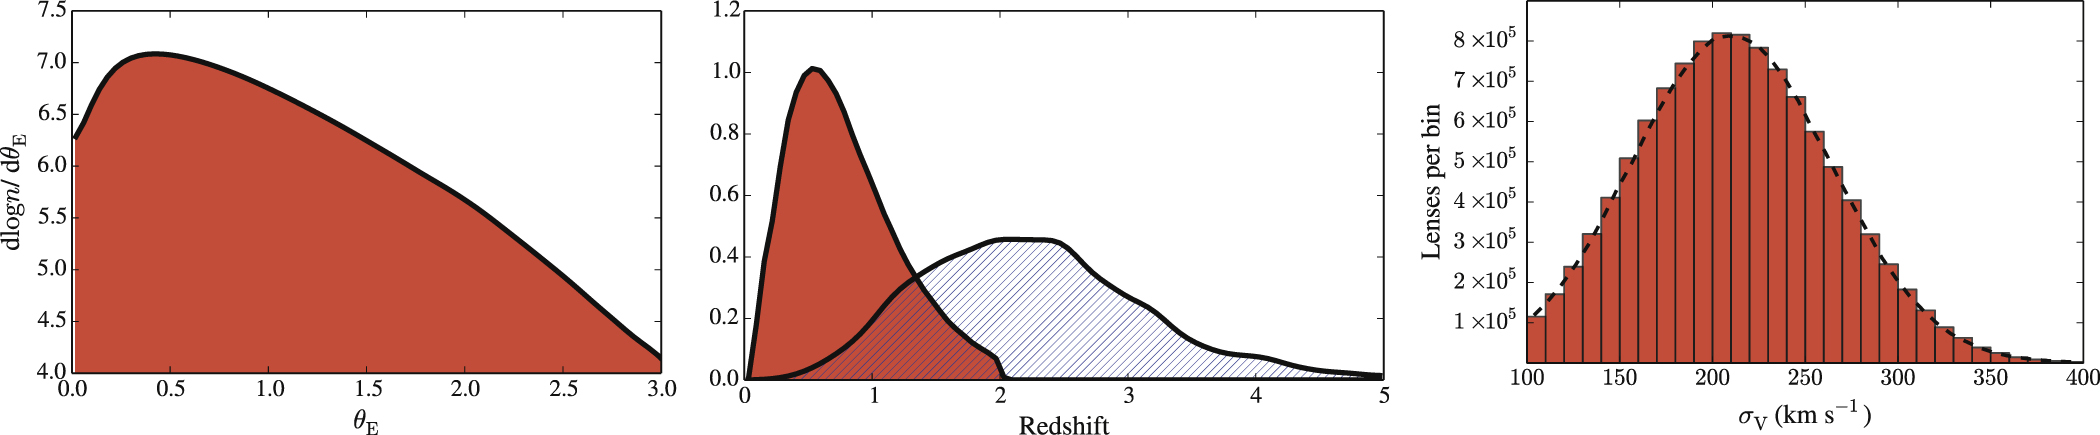
\includegraphics[width=\linewidth]{Immagini//2-Lensing/Collett-1.png}
    \caption{Proprietà di un campione di lenti forti ideale. Da sinistra verso destra, distribuzione del raggio di Einstein dei sistemi, del redshift di sorgenti (grigio) e lenti (rosso) e della dispersione di velocità della lente. Immagine riprodotta da \textcite{Collett2015}.}
    \label{fig:Collett1}
\end{figure}
Si può osservare che la popolazione delle lenti gravitazionali è caratterizzata da galassie  poste per la maggior parte a redshift $0.1 \lesssim z \lesssim 1$, con un picco di dispersione di velocità attorno ai $210$ km/s. Le sorgenti, invece, hanno un picco a redshift $z \simeq 2$. Tali sistemi generano raggi di Einstein dell'ordine di $0.5''$ e, dal primo grafico a sinistra, la distribuzione mostra che i sistemi con raggi di Einstein grandi sono progressivamente più rari. 
La distribuzione in funzione del redshift è determinata anche dal rapporto fra le grandezze geometriche del sistema, come le distanze $D_d, D_s\ \text{e}\ D_{ds}$; poiché esse entrano nella definizione della densità superficiale critica (Eq. \ref{eq:sigma_c}),  $\Sigma_c$ determina per quali redshift della lente si ha il massimo effetto a parità di redshift della sorgente e viceversa.
Le galassie che producono strong lensing sono dunque prevalentemente galassie ellittiche massicce; ciò le rende un campione ideale per studiarne la distribuzione di massa. 

Tuttavia, non tutti i sistemi di strong lensing sono chiaramente osservabili. Lo stesso studio, infatti, ha simulato come la medesima lente fosse vista da telescopi diversi, giungendo ai risultati riportati in Figura \ref{fig:Collett2}.
\begin{figure}
    \centering
    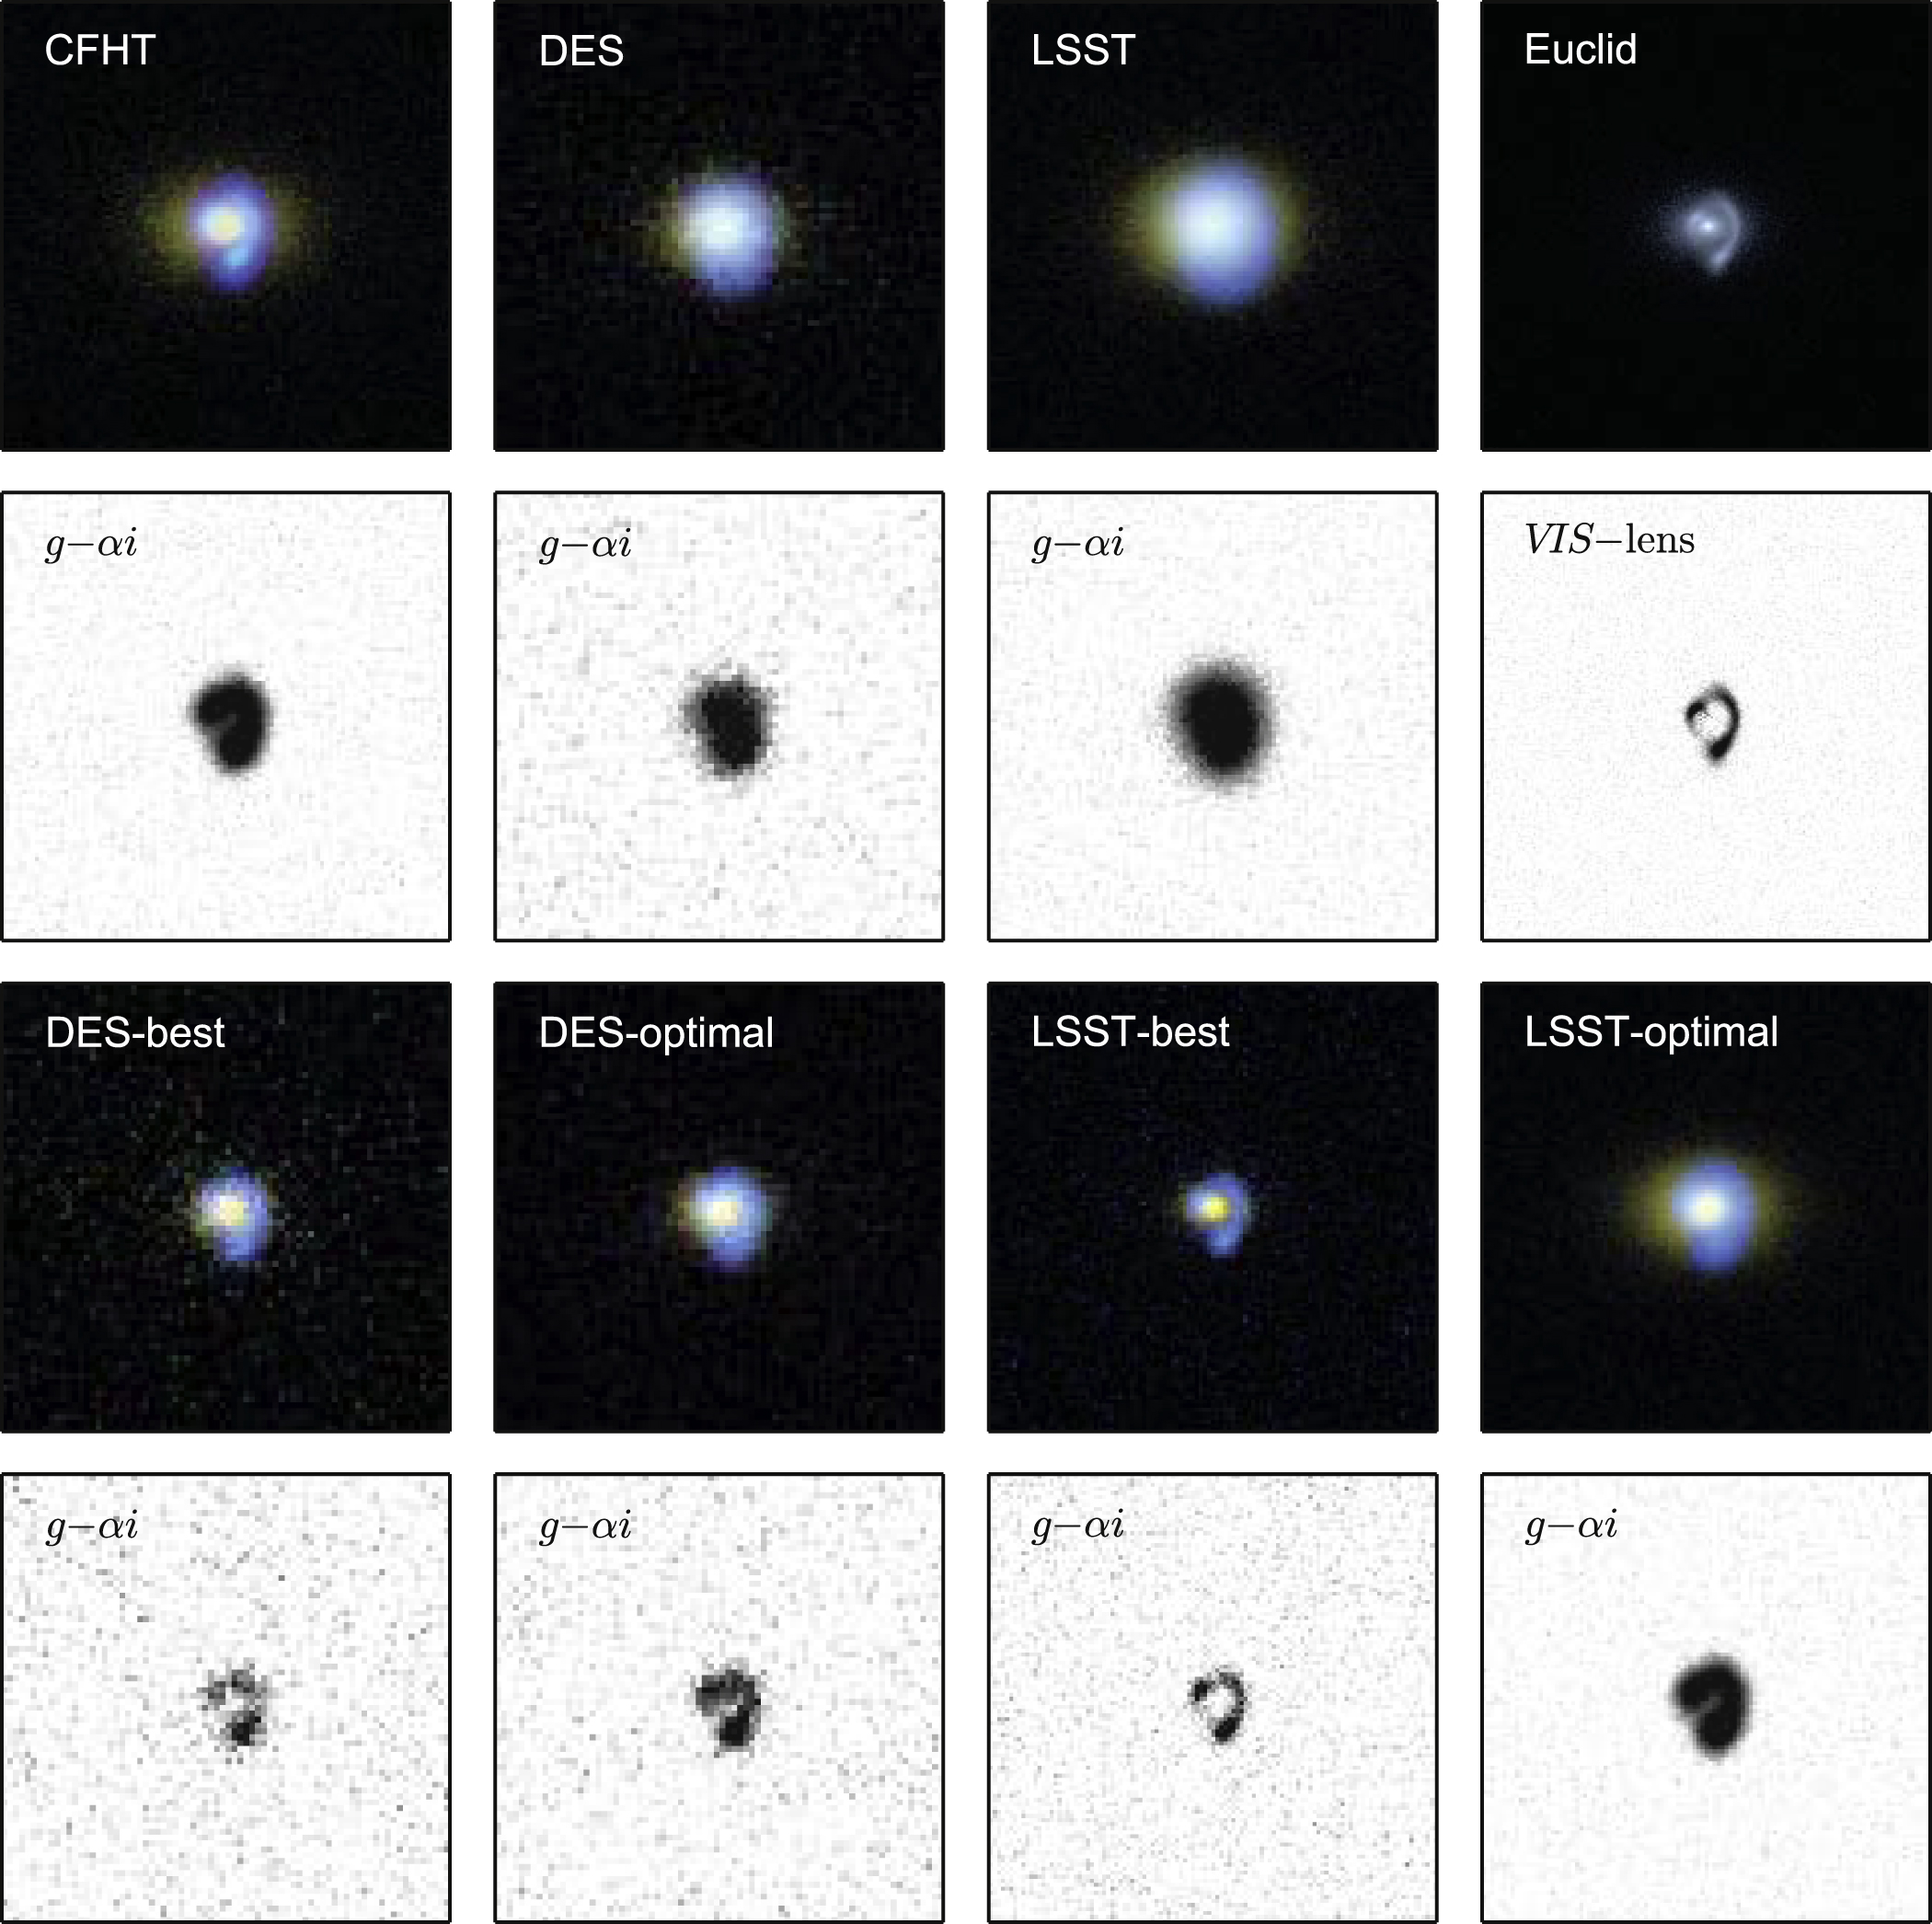
\includegraphics[width=0.60\linewidth]{Immagini//2-Lensing/Collett-2.png}
    \caption{Simulazione di come una stessa lente è osservata da telescopi diversi. Le immagini in bianco e nero sono ottenute mediante filtri particolari, e corrispondono a quelle a colori sovrastanti. Immagine riprodotta da \textcite{Collett2015}. }
    \label{fig:Collett2}
\end{figure}
Se la risoluzione del telescopio è scarsa, gli archi gravitazionali possono diventare quasi indistinguibili dalla lente, rendendo impossibile l'identificazione del sistema di strong lensing pur avendolo osservato. La qualità osservativa è dunque un parametro importante per identificare una lente e modellarne accuratamente la distribuzione di massa. 

Una volta individuati sistemi di strong lensing sufficientemente ben risolti, essi possono essere modellati per ricostruire la distribuzione di massa della galassia lente. Uno dei campioni più studiati è quello della Sloan Lens ACS Survey (SLACS), sfruttato da \textcite{Auger_2010} per analizzare il profilo di massa totale delle galassie ellittiche.
Gli autori utilizzano un campione di \emph{early-type galaxies} (ETGs, galassie primordiali) che danno origine a fenomeni di strong lensing per studiare le relazioni di scala delle ETGs, concentrandosi sulle relazioni tra massa totale, massa stellare e altri parametri strutturali delle lenti.
In particolare, essi confrontano il campione SLACS con il precedente \emph{Sloan Digital Sky Survey} (SDSS), per capire se il loro campione è rappresentativo delle galassie ellittiche massicce. 

In primo luogo viene confrontata la dispersione di velocità stellare entro metà raggio efficace in funzione della distribuzione di massa stellare, ottenendo la Figura \ref{fig:Auger1}.
\begin{figure}
    \centering
    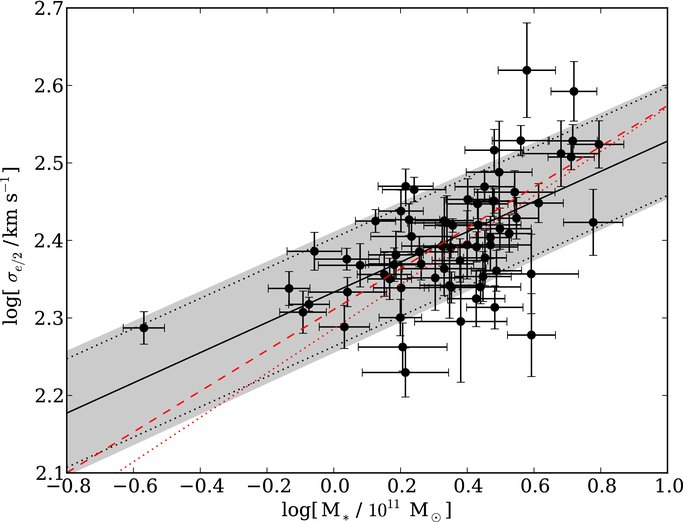
\includegraphics[width=0.75\linewidth]{Immagini//2-Lensing/Auger1.png}
    \caption{Relazione $\sigma_{e/2}-M_\star$ per le lenti SLACS. La linea nera è il fit lineare dei dati, di cui la banda grigia indica l'incertezza. Le linee rosse, invece, rappresentano fit lineari ottenuti in precedenza da altre osservazioni. Le relazioni SLACS risultano essere in accordo con SDSS. Immagine riprodotta da \textcite{Auger_2010}.}
    \label{fig:Auger1}
\end{figure}
Si può notare che esiste con buona approssimazione una relazione lineare tra $\sigma_{e/2}$ e $M_\star$, dunque in generale galassie più massicce hanno dispersioni di velocità più elevate. Ciò è in linea con quanto ci si aspetta da normali ETGs, dunque le galassie lente presentano la stessa relazione massa-dispersione delle normali ellittiche.

Confrontando invece la relazione tra la massa stellare ed il raggio efficace, gli autori hanno ottenuto i risultati riportati in Figura \ref{fig:Auger2}.
\begin{figure}
    \centering
    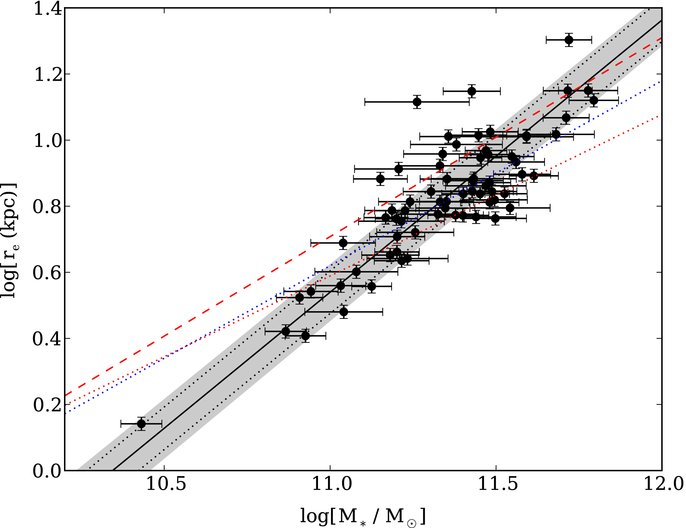
\includegraphics[width=0.75\linewidth]{Immagini//2-Lensing/Auger2.png}
    \caption{Relazione $r_e-M_\star$ per le lenti SLACS. La linea nera è il fit lineare dei dati, di cui la banda grigia indica l'incertezza. Le linee rosse e blu, invece, rappresentano fit lineari ottenuti in precedenza da altre osservazioni. Le relazioni SLACS risultano avere una pendenza maggiore di SDSS, in quanto il campione è in media più massiccio. Immagine riprodotta da \textcite{Auger_2010}.}
    \label{fig:Auger2}
\end{figure}
In generale si può notare che galassie più massicce tendono ad avere anche dimensioni maggiori. Confrontando il fit ottenuto dal campione SLACS con il fit SDSS si nota che gli oggetti SLACS occupano la parte più alta della distribuzione SDSS: la pendenza del fit risulta dunque più ripida non perché le galassie lente siano diverse, ma perché hanno per la maggior parte massa $M_\star > 10^{11}\ M_\odot$. Il campione è dunque rappresentativo delle ellittiche più massicce dell'Universo locale.
Poiché il campione SLACS risulta rappresentativo delle normali ETGs massicce, le proprietà del profilo di massa ricavate dalle lenti possono essere interpretate come proprietà fisiche della popolazione galattica, e non come effetti dovuti alla selezione del campione. 
Una volta verificata la rappresentatività del campione, gli autori combinano le osservazioni di strong lensing con le misure della dinamica stellare per ricostruire il profilo di massa totale delle galassie, vincolandolo a
\begin{equation}
    \rho(r)\propto r^{-\gamma'}
\end{equation}
con pendenza media $\langle \gamma' \rangle=2.028 \pm 0.027$, lievemente maggiore di quella del SIE che prevede $\gamma =2$, ma in buon accordo con esso.

Tale andamento è stato confermato più recentemente anche da \textcite{Shajib2024}. Tuttavia, in quest'ultima review viene anche sollevata la cosiddetta \emph{bulge-halo conspiracy}. La massa totale, infatti, è la somma di due contributi: la massa stellare e la massa di materia oscura. Tuttavia, nessuna delle due singolarmente è isoterma: le stelle seguono circa un profilo de Vaucouleurs ($I(r)\propto r^{\frac{1}{4}}$, dove I è la brillanza superficiale), mentre gli aloni di DM seguono un profilo NFW (Eq. \ref{eq:NFW}). La conoscenza del profilo di massa totale costituisce il punto di partenza per tentare di separare il contributo della componente stellare da quello dell'alone di materia oscura, operazione che richiede ulteriori informazioni osservative e opportune modellizzazioni.

La ricostruzione del profilo di massa totale richiede quindi di modellare il sistema di strong lensing a partire dalle osservazioni. È pertanto necessario comprendere quali informazioni siano effettivamente contenute nelle immagini e quali degenerazioni limitino il recupero dei parametri fisici della lente.

\subsection{Osservabili e degenerazioni principali}
In un sistema di strong lensing, si possono distinguere due categorie di osservabili principali.
La prima sono archi gravitazionali e anelli di Einstein (per sorgenti estese) oppure immagini multiple (per sorgenti puntiformi).
Le diverse manifestazioni delle lenti forti, come analizzato nel paragrafo \ref{sez:Image formation}, dipendono dalla posizione della sorgente rispetto alle caustiche della lente. Alcuni esempi sono presentati in Figura \ref{fig:strong_lenses}.
\begin{figure}
    \centering
    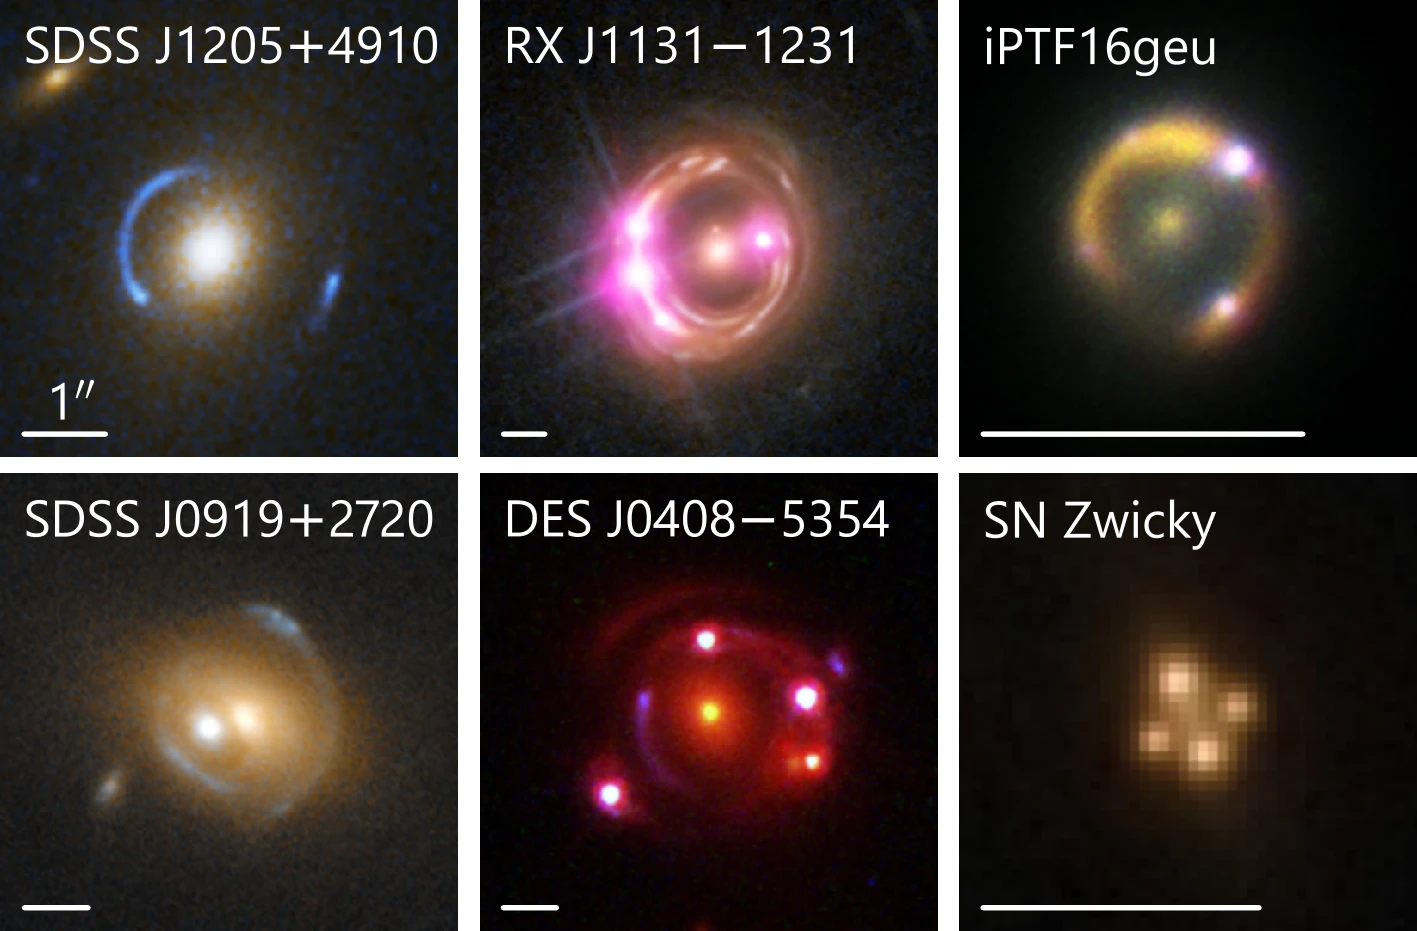
\includegraphics[width=0.7\linewidth]{Immagini//2-Lensing/strong_lenses.png}
    \caption{Esempi fenomenologia di lenti forti su scala galattica, ognuno con sorgenti diverse. Nella prima colonna non è stato possibile risolvere la sorgente; nella seconda e nella terza si hanno rispettivamente immagini di quasar e supernovae. La barra bianca indica una scala di 1''. Figura riprodotta da \textcite{Shajib2024}.}
    \label{fig:strong_lenses}
\end{figure}

Da queste osservabili si possono ricavare vincoli sul potenziale della lente, dunque anche sulla sua distribuzione di massa. Se la sorgente è estesa, ogni pixel dell'arco costituisce un vincolo aggiuntivo sul modello della lente. Se invece è puntiforme, il fatto di poter osservare anche i rapporti e le anomalie di flusso permette di ricavare le magnificazioni e individuare sub-aloni di materia oscura altrimenti invisibili.

La seconda categoria è quella dei ritardi temporali. Se la sorgente è variabile nel tempo, come accade per quasar e supernovae, le immagini variano ad istanti diversi, poiché il percorso verso la posizione sul piano della lente differisce leggermente in base al raggio considerato. Misurando tali ritardi è possibile ottenere un ulteriore vincolo sul potenziale gravitazionale e su parametri cosmologici come $H_0$.

Tuttavia, osservare perfettamente una lente non significa conoscere univocamente la distribuzione di massa. Modelli anche molto diversi fra loro possono infatti dare origine a immagini praticamente identiche, creando una degenerazione. 

La degenerazione più significativa dal punto di vista della ricostruzione del profilo di massa totale è la \emph{Mass-Sheet Degeneracy} (MSD). 
Osservando le immagini create dalla lente è possibile costruire un modello della distribuzione di massa che le riproduca. Tuttavia, esso non è univoco: esiste infatti un'intera famiglia di modelli che produce praticamente gli stessi osservabili di imaging. 
Matematicamente, tale famiglia è descritta dalla trasformazione
\begin{equation}
    \kappa \to \kappa'=\lambda \kappa + 1 - \lambda
\end{equation}
dove $\lambda $ è una costante ed il termine $1-\lambda$ rappresenta una distribuzione uniforme di massa antistante la lente (infatti mass-sheet indica un "foglio" di densità di massa costante). Tale trasformazione implica uno shift anche nella posizione della sorgente 
\begin{equation}
    \beta \to \beta'=\lambda \beta
\end{equation}

Per scegliere il modello corretto, è necessaria un'osservazione indipendente, ad esempio tramite la cinematica stellare. 
Le stelle infatti si muovono nel potenziale gravitazionale reale, ed in generale distribuzioni di massa diverse prediranno dispersioni di velocità diverse. Data una serie di distribuzioni di massa compatibili con le immagini, la cinematica permette dunque di eliminare quelle incompatibili con il moto delle stelle, dando informazioni complementari al lensing e permettendo di eliminare eventuali degenerazioni o di ridurle. Negli studi moderni, i due metodi sono dunque spesso analizzati insieme, in quanto il primo è sensibile alla massa proiettata, mentre il secondo è sensibile alla profondità della buca di potenziale; combinando le informazioni è possibile ricostruire il profilo di massa totale (e di conseguenza anche i contributi singoli di stelle e DM) con un'affidabilità più elevata.

Lo strong lensing permette dunque di ricostruire il profilo di massa totale della galassia lente, a cui contribuiscono sia la parte stellare che la materia oscura. Tuttavia, esse non possono essere osservate separatamente: la distinzione dei singoli contributi richiede ulteriori modelli e informazioni osservative. Indipendentemente da ciò, il lensing è sensibile anche a piccole irregolarità del potenziale gravitazionale. Esse sono utilizzate per indagare la sotto-struttura degli aloni di DM, anche quando la deflessione luminosa è appena percettibile.
Lo strong lensing è dunque uno degli strumenti più potenti per investigare la natura della materia oscura, come verrà approfondito nel capitolo successivo.